\newpage
\chapter{Odstranění knihoven Cg toolkit, OpenGL z programu}
Program DicomPresenter stojí na knihovně OpenGL, používá jí k vykreslování grafického výstupu. Pomocí OpenGL jsou uloženy zobrazované snímky v paměti. Pomocí souřadnicového systému OpenGL pak vykresluje snímky na obrazovku. OpenGL tak slouží ke správě grafických dat a dále díky OpenGL má program nadprůměrně plynulý chod - rychlost vykreslování nad 100fps.

V programu byla dále použita knihovna Cg toolkit. Autor práce \cite{neskudla} obhajuje její použití tím, že v OpenGL se mu nedaří realizovat změnu jasu a kontrastu, a tak k tomuto používá Cg toolkit.

Tato kapitola má za cíl odpovědět na otázku, zda by bylo možné z programu odstranit knihovny OpenGL a Cg toolkit a dále, jaký dopad by to mělo na chod programu. V první části kapitoly autor práce vysvětluje, co je to změna jasu a kontrastu. OpenGL, ani Cg toolkit nenabízejí pro změnu kontrastu předem naprogramované funkce a tak je třeba toto realizovat vlastním kódem. V druhé části kapitoly je pak popsáno, jak byl testován výkon počítače při dílčích úlohách řešených bez použití a s použitím OpenGL. Jednou úlohou je změna kontrastu, druhou úlohou je posunování snímku po obrazovce. Obě tyto úlohy vyplívají z funkčnosti programu DicomPresenter. Změna kontrastu i posunování snímků jsou v DicomPresenteru řešeny real-time, tzn. program okamžitě reaguje na akce uživatele. Pro to, aby bylo možné odstranit knihovnu OpenGL z programu, musíme být schopni bez této knihovny realizovat obě úlohy alespoň 30x za sekundu. Pro odstranění knihovny Cg toolkit z programu musíme být schopni realizovat změnu jasu a kontrastu v OpenGL (případně pak i v C++ bez využití OpenGL).

\subsection{Jas  a kontrast}
Pro to abychom mohli programovat změnu kontrastu v OpenGL, Cg, nebo C++ musíme vědět o jaké matematické operace s pixely snímku se jedná. Popsat změnu kontrastu matematicky si klade za cíl první část této kapitoly.

 V našem případě se můžeme omezit jen na černobílé snímky, protože výstupem MRI jsou pouze černobílé snímky. Obrázek tedy můžeme chápat jako matici čísel mezi $0$ a $1$, kde sloupce, respektive řádky odpovídají souřadnicím bodu v obrázku:

$
 Im_{res_{x},res_{y}} =
 \begin{pmatrix}
  Im(1,1) & Im(1,2) & \cdots & Im(1,res_{x}) \\
  Im(2,1) & Im(2,2) & \cdots & Im(2,res_{x}) \\
  \vdots  & \vdots  & \ddots & \vdots  \\
  Im(res_{y},1) & Im(res_{y},2) & \cdots & Im(res_{y},res_{x})
 \end{pmatrix}
$, $ Im(x,y) \in [0,1] $

Pro $ Im(x,y) = 0 $ vidíme pixel naprosto černý, pro $ Im(x,y) = 1 $ vidíme pixel bílý.

Jas a kontrast lze pak definovat\cite{wikipediaContrast}:


$Brightness(Im) = \frac{1}{res_{x} \cdot res_{y}}\sum_{\substack{0 \leq x \leq res_{x} \\ 0 \leq y \leq res_{y}}} Im(x,y)$

$Contrast(Im) = \sqrt{\frac{1}{res_{x} \cdot res_{y}}\sum_{\substack{ 0 \leq x \leq res_{x} \\ 0 \leq y \leq res_{y} }}(Im_{x,y}-Brightness(Im))^2}$

Jak vidíme ze vzorečků: ten pro jas nápadně připomíná výpočet střední hodnoty; vzoreček pro kontrast pak připomíná výpočet rozptylu.

Pro změnu jasu a kontrastu snímku se pak v počítačových programech používají následující dvě funkce:

$ Im(x,y) \longmapsto Im(x,y) + c_{brightness} $ \\
\indent$ Im(x,y) \longmapsto   (Im(x,y) - 0.5) \cdot c_{contrast} + 0.5 $ \\
\indent kde hodnoty větší než 1 jsou zarovnány na 1 a hodnoty menší než 0 jsou zarovnány na 0.

Bohužel při těchto transformacích dochází ke ztrátě informace v nejsvětlejších a nejtmavších místech obrázku. To se dá řešit použitím složítějších funkcí pro transformace. V tabulce\ref{kontrast} vidíme porovnání lineární a nelineární změny kontrastu.

\noindent
\begin{table}[ht]
	\label{kontrast}
	\centering
		\begin{tabular}{p{0.44\textwidth}p{0.44\textwidth}}
			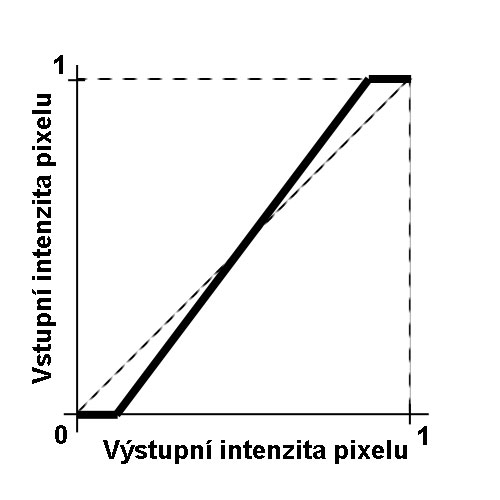
\includegraphics[width=0.4\textwidth,height=0.4\textwidth]{Text/IMG/Kontrast_Transformace_1.jpg}
		&
			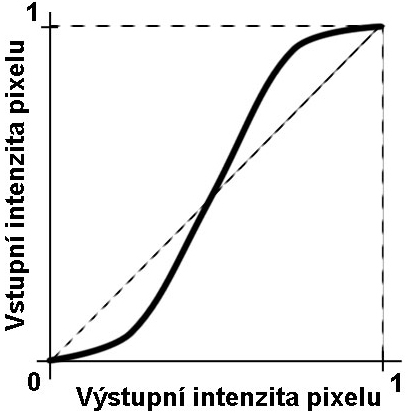
\includegraphics[width=0.4\textwidth,height=0.4\textwidth]{Text/IMG/Kontrast_Transformace_2.jpg}
		\end{tabular}
	\caption{Změna kontrastu pomocí lineární (vlevo) a nelineární (vpravo) transformace. V prvním případě dochází a ve druhém nedochází ke ztrátě informace.}
\end{table}



\subsection{Kontrast nelineárním způsobem}
S využitím jazyka Cg (případně C++ při odstranění OpenGL) lze implementovat nelineární změnu kontrastu zachovávající všechny informace v obrázku. V následující stati najdeme jednu z možných funkcí pro tuto transformaci.

Cílem je najít matematickou funkci, jež se svým grafem blíží grafu v tabulce \ref{kontrast} vrpavo. Podobný průběh má funkce $tanh(c\cdot x)$ na intervalu $(-\infty,\infty)$, kde parametr $c$ určuje derivaci v bodě $0$.

Graf funkce posuneme do bodu  $[\frac{1}{2},\frac{1}{2}]$:

\begin{equation}
f(x) = tanh(c\cdot(x-\frac{1}{2})) + \frac{1}{2}
\end{equation}

Omezíme obor hodnot na interval: $[0,1]$:

\begin{equation} \label{tanh1}
f(x) = \frac{1}{2}\cdot tanh(2\cdot c\cdot(x-\frac{1}{2})) + \frac{1}{2}
\end{equation}

Graf funkce \ref{tanh1} neprochází body $[0,0]$, $[1,1]$. Proto přičteme k funkci jednoduchou lineární funkci:

\begin{equation}
f(x) = k\cdot(x-\frac{1}{2}) + \frac{1}{2}\cdot tanh(2\cdot c\cdot(x-\frac{1}{2})) + \frac{1}{2}
\end{equation}

Lze odvodit, že ke splnění podmínek: $f(0)=0$ a $f(1)=1$ je třeba aby:

\begin{equation}
k = 1 - tanh(c)
\end{equation}

Dosazením dostáváme výsledný tvar funkce:

\begin{center}
\framebox{ $f(x) = (1 - tanh(c))\cdot(x-\frac{1}{2}) + \frac{1}{2}\cdot tanh(2 \cdot c\cdot(x-\frac{1}{2})) + \frac{1}{2} $ }
\end{center}

V tabulce \ref{kontrast} vidíme graf pro c=1 a c=2.


\noindent
\begin{table}[ht]
	\label{kontrast}
	\centering
		\begin{tabular}{p{0.3\textwidth}p{0.3\textwidth}}
			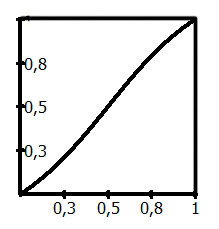
\includegraphics[width=0.3\textwidth,height=0.3\textwidth]{Text/IMG/nelinearni1.jpg}
		&
			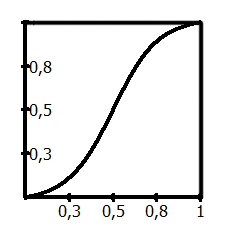
\includegraphics[width=0.3\textwidth,height=0.3\textwidth]{Text/IMG/nelinearni2.jpg}
		\end{tabular}
	\caption{Graf nalezené funkce pro nelineární změnu kontrastu pro $c=1$ (vlevo) a $c=2$ (vpravo).}
\end{table}


\newpage
\subsection{Kontrast a světlost v OpenGL}
Pro realizaci jednoduchých barevných transformací snímku disponuje knihovna OpenGL funkcemi Bias a Scale.

\begin{itemize}
\item Voláním funkce Bias s parametry K,B provedeme přičtení konstanty K k hodnotě barevné složky B pro všechny pixely obrázku.
\item Voláním funkce Scale s parametry K,B provedeme vynásobení stávající barevné složky B konstantou K pro všechny pixely obrázku.
\end{itemize}

Transformační křivky obou funkcí vidíme v tabulce \ref{biasscale}. Funkce Bias odpovídá změně jasu snímku. Změnu kontrastu musíme realizovat pomocí volání obou funkcí se správně dopočítanými parametry.

Pro změnu kontrastu voláme nejdřív funkci Scale s parametrem $s$, pak funkci Bias s parametrem $b$. Výsledek odpovídá transformaci:
 
\framebox{ $ y = s \cdot x + b$ }

Vztah mezi parametry $b$ a $s$ takový, aby transformační křivka procházela bodem [0.5,0.5], je:

\framebox{ $b=\frac{1}{2}\cdot(1-s)$ }

\noindent
\begin{table}[ht]
	\label{biasscale}
	\centering
		\begin{tabular}{p{0.35\textwidth}p{0.35\textwidth}}
			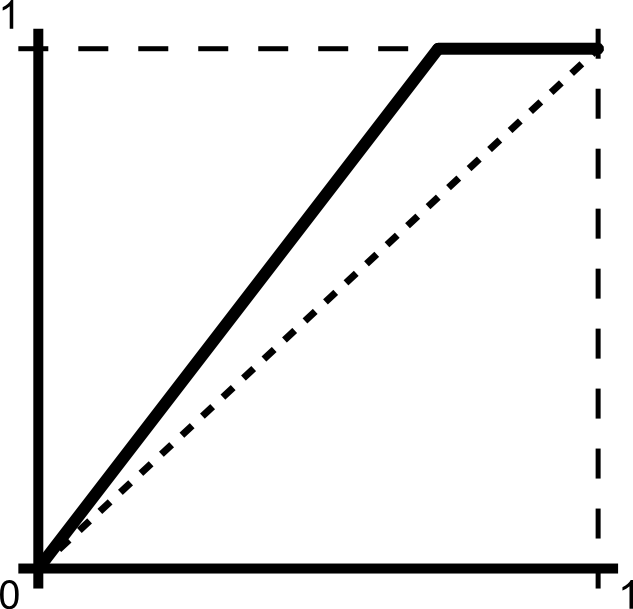
\includegraphics[width=0.3\textwidth]{Text/IMG/Bias.png}
		&
			\includegraphics[width=0.3\textwidth]{Text/IMG/Scale.png}
		\end{tabular}
	\caption{Křivka transformací Bias (vlevo) a Scale (vpravo). Jejich správnou kombinací lze dosáhnout změny kontrastu.}
\end{table}

<< neskudla >>




\begin{comment}
\subsection{Kontrast v knihovně Cg toolkit}
Knihovna Cg toolkit nabízí oproti OpenGL programování výpočtů s barevnými složkami. Pomocí funkce tex2D si zjistíme barevné složky původního pixelu, s nimi pak můžeme provádět libovolné operace a výsledek pak uložit do výstupu.
\subsection{Kontrast lineární transformací}
Knihovna Cg opět nedisponuje funkcí pro změnu kontrastu, ale podobně jako v předchozím případě si můžeme změnu kontrastu naprogramovat sami - v tomto případě mnohem přehlednějším způsobem. Násobme barevné hodnoty pixelu koeficientem a přičtěme adekvátní konstantu. To v Cg zapíšeme takto:
\begin{lstlisting}[label=DicomImageClass,caption={...}]
C3E3f_Output main(float2 texCoord : TEXCOORD0, uniform sampler2D decal : TEX0, uniform float brightness){
  C3E3f_Output OUT;
  OUT.color = tex2D(decal,texCoord)*scale + bias;
  return OUT;
}
\end{lstlisting}
Ve srovnání s OpenGL je tato implementace výrazně přehlednější. Podíváme-li se na řádek 3, vidíme hned zápis transformační funkce ve tvaru: f(x) = k*x - z. 
Změna jasu pak bude provedena přičtením konstanty bez násobení: \clist{OUT.color = tex2D(decal,texCoord)*scale}.
\end{comment}





\section{Rychlost vykreslování}
Jednou z otázek na kterou se snaží najít odpověď tento VÚ je to, zda by bylo možné z programu odstranit knihovny OpenGL a Cg toolkit. Jedná se o knihovny zajišťující práci s grafickými daty, hlavně se pak jedná o knihovnu výrazně urychlující zobrazování grafických dat. Před odstraněním knihoven z programu musíme nejprve zjistit, zda bude možné realizovat zobrazování dodstatečně rychle i bez těchto knihoven. 

Při vývoji DicomPresenteru byl kladen důraz na dostatečně plynulé ovládání. Pro práci s jakoukoliv aplikací je pohodlné, je-li mezi uživatelskou akcí a její realizací co nejkratší prodleva. V DicomPresenteru jsou výpočetně nejnáročnejčí akce: přesouvání snímků po obrazovce, úprava jasu a kontrastu snímků. Průměrný počet vykreslených snímků za sekundu při těchto akcích je při využití OpenGL 90 fps. Odhad toho, jak rychle poběží program bez OpenGL a Cg toolkit můžeme udělat tak, že naprogramujeme dvě aplikace, které budou mít na starosti pouze dvě zmiňované akce (posun snímku, změnu kontrastu). Jeden program bude využívat knihovny, druhý ne. Výkon testovacích aplikací a DicomPresenteru se bude jistě značně lišit\footnote{Rozdíl v rychlosti vykreslování u DicomPresenteru a testovacích aplikací je způsoben tím, že DicomPresenter vedle vykreslování dat na obrazovku musí řešit další úlohy: zachytávání uživatelských akcí, předávání uživatelských akcí napříč objektovým modelem, vykreslování ovladacích prvků, vykreslování textů.}, ale z naměřených hodnot lze odhadnout, jak rychle poběží DicomPresenter bez OpenGL a Cg toolkit. Uvažujme nyní pouze jednu z úloh: označme si $fps_{lib}$ počet naměřených snímků za sekundu v aplikaci využívající knihovny, $fps_{software}$ počet naměřených fps v aplikaci nevyužívající grafické knihovny, $fps_{dp}$ nechť je průměrný počet snímků kterého dosahuje DicomPresenter. Pak spodní odhad\footnote{Vykreslování na obrazovku je jen část úloh, které DicomPresenter řeší v každém kroku. Zpomalíme-li tuto část n-krát, bude pak běh programu v nejhorším případě n-krát pomalejší.} průměrného počtu snímků, kterého bude dosahovat DicomPresenter bez OpenGL a Cg toolkit v dané úloze je:

\begin{equation}
fps_{odhad} = \frac{fps_{software}}{fps_{lib}} \cdot fps_{dp}
\end{equation}

\subsection{Změna kontrastu bez Cg toolkit}

\begin{lstlisting}[label=DicomImageClass,caption={...}]
for (int y = 0; y<h; y++){
	Rgb = (QRgb*)ShowImage.scanLine(y);
	for ( int x = 0; x < w; x++ ){
		Rgb[x] = qRgb(qRed(Rgb[x])*c+0.5*(1-c),qGreen(Rgb[x])*c+0.5*(1-c),qBlue(Rgb[x])*c+0.5*(1-c));
	}
}
\end{lstlisting}

\subsection{Změna kontrastu v Cg toolkit}

\begin{lstlisting}[label=DicomImageClass,caption={...}]
C3E3f_Output main(float2 texCoord :TEXCOORD0, uniform sampler2D decal :TEX0, uniform float contrast){
  C3E3f_Output OUT;
  OUT.color = tex2D(decal,texCoord)*contrast+0.5(1-contrast);
  return OUT;
}
\end{lstlisting}

\subsection{Posun snímku bez OpenGL}
\begin{lstlisting}
void Workspace::draw(QPoint leftTop, QImage *sourceImage){
	int width = sourceImage->width();
	int height = sourceImage->height();
	int xPos = leftTop.x();
	int yPos = leftTop.y();
	for ( int y = 0; y < this->height(); y++ ){
		QRgb *workspaceImageLinePtr = (QRgb*)this->scanLine(y);
		for ( int x = 0; x < this->width(); x++ ){
			workspaceImageLinePtr[x] = qRgb(0,0,0);
		}
	}
	for ( int y = 0; y < height; y++ ){
		QRgb *sourceImageLinePtr = (QRgb*)sourceImage->scanLine(y);
		QRgb *workspaceImageLinePtr = (QRgb*)this->scanLine(yPos + y);
		for ( int x = 0; x < width; x++ ){
			workspaceImageLinePtr[xPos + x] = qRgb(qRed(sourceImageLinePtr[x]),qGreen(sourceImageLinePtr[x]),qBlue(sourceImageLinePtr[x]));
		}
	}
}
\end{lstlisting}

\subsection{Posun snímku s OpenGL}

\begin{lstlisting}
void GLPainter::Paint(int translationX){
	glClear(GL_COLOR_BUFFER_BIT);
	float ratio = (float)translationX/im->width().;
	glBegin(GL_POLYGON);
		glColor3f (Brightness, Brightness, Brightness);
		glTexCoord3f(0.0,0.0,0.0);	glVertex3f(ratio+ -1.0, -1.0, 0.0 );
		glTexCoord3f(0.0,1.0,0.0);	glVertex3f(ratio+ -1.0,  1.0, 0.0 );
		glTexCoord3f(1.0,1.0,0.0);	glVertex3f(ratio+  0.0,  1.0, 0.0 );
		glTexCoord3f(1.0,0.0,0.0);	glVertex3f(ratio+  0.0, -1.0, 0.0 );
	glEnd();
}
\end{lstlisting}






























\begin{comment}

\subsection{Implementace v Qt}
Grafická část rozhraní knihovny Qt je dělaná čistě pro dvojrozměrnou grafiku a všechny výpočty jsou prováděny jen na procesoru. Chceme-li měnit světlost snímku, musíme procházet for-cyklem všechny body obrázku a provést operaci pro každý bod zvlášť. Pokud navíc zadáme světlost pixelu mimo požadovanou mez, program se zasekne. Narozdíl od toho knihovny OpenGL i Cg automaticky barevnou hodnotu pixelu oříznou na přípustnou mez.

Intuitivní, avšak pomalejší implementace v Qt knihovně vypadá následovně:

\begin{lstlisting}[label=DicomImageClass,caption={...}]
for (int y=0; y<h; y++){
	for (int x=0; x<w; x++){
		Rgb = MemoryImage.pixel(x,y);
		Rgb = qRgb(qRed(Rgb)*cont,qGreen(Rgb)*cont,qBlue(Rgb)*cont);
		ShowImage.setPixel(x,y,Rgb);
	}
}
\end{lstlisting}

V úryvku kódu vidíme zejména procházení celého obrázku ve dvou for-cyklech(řádky 13,14). V každém kroku si zjistíme barevné souřadnice pixelu, upravíme je a uložíme je. To má na starosti procesor a jedná se o největší handicap celého programu. Při této implementaci je úloha zpracována sériově na jednom jádře, jak je vidět z následujících grafů sledujících zátěž jednotlivých jader:

\hspace{1cm}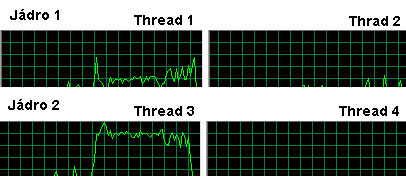
\includegraphics[width=0.8\textwidth]{Text/IMG/MultiThread.jpg}

Procesor je fyzicky dvoujádrový, ale operační systém jej vidí jako čyřjádrový. Celý výpočet probíhal viditelně v třetím threadu, v prvním pak běžely zřejmě jen pomocné operace, další 2 thready zůstaly nevyužité.

Chceme-li výpočet urychlit, můžeme tak udělat v několika krocích:

Nebudeme si ukládat barevné souřadnice původního obrázku do proměnné, tam je upravovat a ukládat zpět na půbodní místo. Ale necháme si předat ukazatel na místo v paměti, kde je obrázek uložen, a výsledek ukládat přímo tam.

Dále nebudeme volat funkci, která nám na základě souřadnic vrátí barevné složky obrázku, ale necháme si od Qt knihovny předat ukazatel na celý jeden řádek obrázku. Tím se vyhneme opakovanému volání funkce.

Dvojice for-cyklů procházející obrázek bude nahrazena tímto kódem:

\begin{lstlisting}[label=DicomImageClass,caption={...}]
for (int y = 0; y<h; y++){
	Rgb = (QRgb*)ShowImage.scanLine(y);
	for ( int x = 0; x < w; x++ ){
		Rgb[x] = qRgb(qRed(Rgb[x])*cont,qGreen(Rgb[x])*cont,qBlue(Rgb[x])*cont);
	}
}
\end{lstlisting}

Jak je vidět, v každém řádku obrázku ušetříme hned dvě volání funkce pro každý pixel. Zkusme si spočítat kolik funkčních volání jsme ušetřili:

V prvním případě voláme pro každý pixel funkce QImage::pixel() a QImage::setPixel(). Rozměr obrázku je 512*512 pixelů. To jest: 512*512*2 = cca 500 000 funkčních volání.

V druhém případě voláme pouze funkci QImage::scanLine pro každý řádek obrázku, tj. 512*2 = 1024 volání.

Jak je vidět, jedná se o zredukování počtu volání nějaké funkce o dva řády. Výsledek takového zjednodušení uvidíme v závěru kapitoly.


\subsection{Implementace v OpenGL}

OpenGL je knihovna přímo určená pro urychlení grafických výpočtů a jejich zjednodušenou obsluhu. Hlavní rozdíl oproti implementaci v Qt je ten, že výpočty neprobíhají na procesoru, ale na grafické kartě, což je, jak se později ukáže, zásadní rozdíl ve výkonnosti programu. Stejně tak data nejsou uložena v modulech paměti RAM na základní desce, ale jsou v paměti grafické karty.

Implementace vypadá následovně:

\begin{lstlisting}[label=DicomImageClass,caption={...}]
start = time (NULL);
for (int j=0; j<10; j++){
	float Brightness=0.0;
	for (int i=0; i<1000; i++){
		Brightness = Brightness+0.001;
		gl->Paint(Brightness);
		w.updateGL();
	}
}
end = time (NULL);

void GLPainter::PrepareTexture() {
	glBindTexture( GL_TEXTURE_2D, TextureIdentifier );
	gluBuild2DMipmaps( GL_TEXTURE_2D, 3, width, height, GL_RGB, GL_UNSIGNED_BYTE, TextureData );
	glEnable( GL_TEXTURE_2D );
}

void GLPainter::Paint(float Brightness){
	glBegin(GL_POLYGON);
		glColor3f (Brightness, Brightness, Brightness);
		glTexCoord3f(0.0,0.0,0.0);	glVertex3f( -1.0, -1.0, 0.0 );
		glTexCoord3f(0.0,1.0,0.0);	glVertex3f( -1.0,  1.0, 0.0 );
		glTexCoord3f(1.0,1.0,0.0);	glVertex3f(  1.0,  1.0, 0.0 );
		glTexCoord3f(1.0,0.0,0.0);	glVertex3f(  1.0, -1.0, 0.0 );
	glEnd();
}
\end{lstlisting}
Na první pohled lze vidět nesrovnatelné zjednodušení kódu, zatímco v prvním případě (Qt) jsme museli procházet celý obrázek po pixelech, zde můžeme využít funkce knihovny OpenGL pomocí které lze měnit světlost jejího výstupu.

V programu si nejprve snímek uložíme do paměti jakožto OpenGL texturu (řádky 12-16), posléze provádíme vykreslování této textury na načrtnutý obdélník (18-26).


\subsection{Iplementace v Cg}

Knihovna Cg slouží k programování výpočtů na čipu grafické karty. V jednoduchém jazyku podobném jazyku C popíšeme prováděné výpočty pro změnu světlosti. Výpočty jsou pak realizovány na speciálním hardwarovém čipu (pixel shader, vertex shader). Přínos pixel a vertex shaderů je v nové paletě efektů, jež je možno provádět, a dále ve výrazném urychlení těchto efektů.

Podívejme se na implementaci programu s využitím Cg, tentokráte výpočty nebyly prováděny jen v prostředí jazyka C++, ale i v jazyce Cg.

\begin{lstlisting}[label=DicomImageClass,caption={...}]
start = time (NULL);
for (int j=0; j<10; j++){
	float Brightness=0.0;
	for (int i=0; i<1000; i++){
		Brightness = Brightness+0.001;
		gl->Paint(Brightness);
		w.updateGL();
	}
}
end = time (NULL);

void GLPainter::PrepareTexture() {
	glBindTexture( GL_TEXTURE_2D, TextureIdentifier );
	gluBuild2DMipmaps( GL_TEXTURE_2D, 3, width, height, GL_RGB, GL_UNSIGNED_BYTE, TextureData );
	glEnable( GL_TEXTURE_2D );
}

void GLPainter::changeBrightness( float Brightness ){
	cgGLBindProgram(Program);
	cgGLEnableProfile(Profile);
	cgSetParameter1f(hBright, Brightness);
	cgUpdateProgramParameters (Program);
	cgGLDisableProfile(Profile);

	Paint();
}

void GLPainter::Paint(){
	glClear(GL_COLOR_BUFFER_BIT);

	cgGLBindProgram(Program);
	cgGLEnableProfile(Profile);
	cgGLEnableTextureParameter(hDecal);

	glBegin(GL_POLYGON);
		glTexCoord3f(0.0,0.0,0.0);	glVertex3f(-1.0,-1.0,0.0);
		glTexCoord3f(0.0,1.0,0.0);	glVertex3f(-1.0,1.0,0.0);
		glTexCoord3f(1.0,1.0,0.0);	glVertex3f(1.0,1.0,0.0);
		glTexCoord3f(1.0,0.0,0.0);	glVertex3f(1.0,-1.0,0.0);
	glEnd();

	cgGLDisableProfile(Profile);
	cgGLDisableTextureParameter(hDecal);
}
\end{lstlisting}

\begin{lstlisting}[label=DicomImageClass,caption={...}]
struct C3E3f_Output {
  float4 color : COLOR;
};

C3E3f_Output main(float2 texCoord : TEXCOORD0, uniform sampler2D decal : TEX0, uniform float brightness)
{
  C3E3f_Output OUT;
  OUT.color = tex2D(decal,texCoord)*brightness;

  return OUT;
}
\end{lstlisting}

První část programu je shodná s předchozí verzí (opět je volána knihovna OpenGL). Rozdíl však začíná od řádku 18. Ve funkci changeBrightness() musíme volat funkce knihovny Cg toolkit pomocí kterých předáme pixel shaderu parametr určující změnu světlosti. Před samotným vykreslováním pomocí OpenGL (řádky 35-40) musíme nechat program zkompilovat na čipu grafické karty a nastavit, aby ovlivňoval výstup OpenGL.

Za povšimnutí stojí fakt, že výpočet změny světlosti se přesunul z kódu C++ do Cg. Změna světlosti je popsána v samostatném programu jež se kompiluje na grafické kartě.


\subsection{Porovnání výpočtů}

Popsané programy byly testovány na počítačové sestavě:

Intel Core i3, ATI Radeon 5470. Takt procesoru je 2,26 GHz

Jedná se o dvoujádrový procesor, pro výpočet však bylo použito pouze jedno jádro. Takt GPU na grafické kartě je 750MHz.

V každé konfiguraci jsme požadovali jiný počet cyklů programu, jenom z důvodu časové úspory při ladění.

\begin{tabular}{| p{5cm} | l | l | l | }
  \hline                       
  Typ konfigurace & Počet cyklů & Čas & Snímků za vteřinu \\
  \hline
  \hline
  Qt (bez přímého přístupu do paměti)& 100 & 4 sekundy & 25 fps\\
  \hline
  Qt (s přímým přístupem do paměti)& 1000 & 11 sekund & 90 fps\\
  \hline
  Qt, OpenGL & 10 000 & 16 sekund & cca 600  fps \\
  \hline
  Qt, OpenGL, Cg & 10 000 & 14 sekund & cca 700 fps \\
  \hline  
\end{tabular}

Jak je vidět z naměřených údajů, s použitím knihovny OpenGL se dá dosáhnout úctihodného výkonu při vykreslování snímků v programu. Nicméně vezmeme-li v úvahu fakt, že standardní rychlost snímání ovládacích zařízení přes USB v operačním systému je 125Hz a dále obnovovací frekvence u monitoru nebývá zpravidla vyšší než 100Hz, musíme uznat, že výkon dosažený pomocí OpenGL je nadbytečný. To by určitě nevadilo a velká rezerva ve výkonu by mohla být zárukou plynulého chodu programu i za ztížených podmínek (uživatel využívá procesor i jiným způsobem za běhu programu), ale bohužel přítomnost knihovny OpenGL v programu má za důsledek značné problémy s provozem programu na méně výkonných, či starších grafických kartách. Byly zjištěny problémy s provozem programu na integrovaných grafických kartách Intel, které však jsou velice často instalovány do moderních notebooků.

Výkon programu, při pomalejší implementaci v Qt knihovně, kdy jsme nevyužívali manuálního přístupu do paměti, ale k tomuto jsme používali implementované funkce v Qt knohovně, je spíše nedostačující. Dosažený výkon v testovacím programu: 25 snímků za vteřinu sice sám o sobě dostačující je, ale musíme vzít v úvahu ten fakt, že se jednalo o velice primitivní testovací program, který nedělal nic jiného než přepočet barevných složek obrázku a jeho zobrazení. DicomPresenter vedle toho musí vykreslovat ovládací prvky programu, což znamená několik funkčních volání navíc.

Oproti tomu výkon dosažený pomocí pokročilé implementace, kdy přistupujeme ručně do paměti počítače a obrazová data měníme tam, by měl být dostačující pro běh reálného programu. I při výrazném zpomalení aplikace kvůli přepočítávání zobrazovaných ovládacích prvků, bychom se měli bezpečně udržet nad hranicí 30FPS.

Závěrem této kapitoly je nutno podotknout, že Knihovny OpenGL, Cg z programu odstranit lze a v nejbližší době bude takto učiněno. Program by se tak měl stát výrazně bezproblémovější, co se týče provozu v praxi. Měl by být kompatibilní s převážnou většinou počítačových sestav - to je však nutná podmínka pro to, aby program mohl být v praxi použitelný.


\end{comment}

\section{}
